\RequirePackage[T1]{fontenc}
\documentclass[conference,letterpaper]{IEEEtran}
\usepackage[spanish,es-nodecimaldot,es-tabla,es-noshorthands]{babel}
\usepackage{amsmath,amssymb,siunitx,booktabs,tabularx}
\usepackage{tikz,circuitikz,pgfplots}
\usetikzlibrary{arrows.meta,positioning,babel}
\usepgfplotslibrary{groupplots}
\pgfplotsset{compat=1.18}
\usepackage{float}
\usepackage[nospread]{flushend}
\usepackage[hidelinks]{hyperref}
\raggedbottom
\interdisplaylinepenalty=2500
\setlength{\emergencystretch}{1em}
\newcolumntype{Y}{>{\centering\arraybackslash}X}
\newcolumntype{L}{>{\raggedright\arraybackslash}X}
\newcommand{\plotstyle}{ }
\begin{document}
\special{pdf:minorversion 7}
\title{Implementación y validación experimental del PI}\author{\IEEEauthorblockN{Martín Ramírez Espinosa, Jerónimo Vargas Orozco\\Andrew Esteban Henao Becerra, Mateo Alexander Cardenas Cuesta}
\IEEEauthorblockA{Universidad Nacional de Colombia, Sede Manizales\\\texttt{maramirezes@unal.edu.co}, \texttt{jevargaso@unal.edu.co}\\\texttt{anhenaobe@unal.edu.co}, \texttt{macardenascu@unal.edu.co}}}
\hypersetup{pdftitle={Implementación y validación experimental del PI},pdfauthor={Martín Ramírez Espinosa, Jerónimo Vargas Orozco, Andrew Esteban Henao Becerra, Mateo Alexander Cardenas Cuesta}}\maketitle
\begin{center}\small Entrega 4: Metodología digital; ensayos pendientes\end{center}
\begin{abstract}Se documenta la integración del PI con ADC y PWM: calibración, temporización, saturación y reajuste. Se establecen cuatro pruebas de aceptación. La integración física, las mediciones y los resultados experimentales permanecen pendientes.\end{abstract}
\section{Alcance}
La guía exige implementar y ajustar el compensador y repetir cuatro ensayos físicos \cite{guide}. La placa está diseñada y el firmware STM32 compila. El código integra adquisición, DMA y PWM, y el núcleo C cuenta con pruebas en computador. Faltan el montaje, la programación del MCU, la calibración y las capturas físicas. No se declara completada la implementación física.

\section{Adquisición y calibración}
El divisor nominal tiene $R_t=3\,\mathrm{k}\Omega$ y $R_b=1\,\mathrm{k}\Omega$. Para un ADC unipolar de $N$ bits:

\begin{equation}\label{eq:adc}\begin{aligned}v_s[k]&=\frac{n_kV_{\mathrm{ADC}}}{2^N-1},\\\hat v_o[k]&=a\,v_s[k]+b,\quad a_{\mathrm{nom}}=1+R_t/R_b=4,\\\Delta v_{o,\mathrm{LSB}}&=\frac{aV_{\mathrm{ADC}}}{2^N-1}.\end{aligned}\end{equation}
Obtener $a,b$ con dos tensiones conocidas y validar con un tercer punto. Medir referencia y resistencias, registrar residuos y comprobar rango del ADC durante transitorios. Comparar resolución efectiva, ruido e incertidumbre con la meta de $20\,\mathrm{mV}$.

La media por periodo requiere varias muestras sincronizadas; una sola muestra no reproduce automáticamente el promedio simulado. La configuración es de 12 bits, referencia nominal de 3.3 V y muestreo de 200 kHz; deben verificarse en la placa real.

\begin{table}[H]\caption{Configurado en firmware; verificación física pendiente}\label{tab:hardware}\centering\footnotesize\setlength{\tabcolsep}{2pt}\renewcommand{\arraystretch}{1.18}\begin{tabularx}{\columnwidth}{LY}\toprule
Dato & Configuración; falta medir\\\midrule
MCU y reloj & STM32F103C8T6; 72 MHz\\
ADC & 12 bits; 3.3 V nominal; 200 kHz\\
Media; filtro & 20 muestras; RC de 0.75 us\\
PWM & 10 kHz; 7200 cuentas\\
Calibración y jitter & Pendiente\\
Instrumentos y fotografía & Pendiente\\\bottomrule\end{tabularx}\end{table}
\section{Algoritmo y temporización}
Se usa $e_k=r_k-\hat v_{o,k}$ y se devuelve $d^{\prime}_k=1-d_k^{\mathrm{cmd}}$. Verificar con osciloscopio la inversión del driver antes de conectar potencia.

\begin{equation}\label{eq:firmware}\begin{aligned}u_k&=0.5+K_pe_k+z_k,\\d_k^{\mathrm{cmd}}&=\operatorname{clip}(u_k,0.05,0.95),\\z_{k+1}&=z_k+\gamma_ke_k,\\\gamma_k&=\begin{cases}0,&u_k\geq0.95,\ e_k>0,\\0,&u_k\leq0.05,\ e_k<0,\\K_iT_s,&\text{en otro caso}.\end{cases}\end{aligned}\end{equation}
La rutina calcula la orden con la integral anterior y luego actualiza el estado. Cada $100\,\mu\mathrm{s}$ completa la media previa y precarga el PWM para el periodo siguiente (Fig.~\ref{fig:timing}). Verificar latencia con un pin de diagnóstico y ausencia de interrupciones perdidas.

\begin{figure}[H]\centering\resizebox{\columnwidth}{!}{\begin{tikzpicture}[font=\footnotesize,>=Stealth]
\draw[->] (0,0) -- (7.6,0) node[right]{$t$};
\foreach \x/\lab in {0/{k-1},2.4/k,4.8/{k+1},7.2/{k+2}} {
\draw (\x,-.1)--(\x,.1) node[above]{$\lab$};}
\draw[<->] (0,-.5)--node[below]{media $\bar v_{k-1}$}(2.4,-.5);
\node[align=center] at (2.4,-1.35) {cálculo\\$d_k^{\mathrm{cmd}}$};
\draw[->] (2.4,-1.8)--node[below]{precarga: $T_s$}(4.8,-1.8);
\draw[<->] (4.8,-.5)--node[below]{$d_k^{\mathrm{cmd}}$ aplicado}(7.2,-.5);
\end{tikzpicture}}\caption{Secuencia que debe reproducir la tarjeta: media, cálculo y aplicación retardada de la orden.}\label{fig:timing}\end{figure}
\begin{table}[H]\caption{Coeficientes diseñados y cargados}\label{tab:coefficients}\centering\footnotesize\setlength{\tabcolsep}{2pt}\renewcommand{\arraystretch}{1.18}\begin{tabularx}{\columnwidth}{LYY}\toprule
Magnitud & Diseño / núcleo C & En tarjeta\\\midrule
$K_p$ ($\mathrm{V}^{-1}$) & 0.026165529 & Pendiente\\
$K_i$ ($(\mathrm{V\,s})^{-1}$) & 78.496586 & Pendiente\\
$K_iT_s$ ($\mathrm{V}^{-1}$) & 0.007849659 & Pendiente\\
$T_s$ ($\mu$s) & 100 & Pendiente\\
$d_{\min}$; $d_{\max}$ & 0.05; 0.95 & Pendiente\\\bottomrule\end{tabularx}\end{table}
El núcleo devuelve $d^{\prime}=1$ al deshabilitarse o enclavar fallo; detecta valores no finitos, tensiones fuera de rango y salida mayor que $8.5\,\mathrm{V}$. Verificar apagado eléctrico real. La rutina no mide corriente ni sustituye la protección de sobrecorriente.

\section{Puesta en marcha y reajuste}
Usar el montaje ya validado en lazo abierto, fuente limitada y referencia gradual. El firmware incorpora rampa de duty y transferencia al PI con ajuste de integral; falta verificarla en hardware. Verificar saturación, recuperación de la integral y apagado antes de alcanzar $6\,\mathrm{V}$.

Si se requiere reajuste, actualizar $G_d$ con parámetros medidos y considerar el retardo real. Recalcular la condición $|K(j\omega_c)G_d(j\omega_c)|=1$, reducir cruce si el margen resulta insuficiente y conservar ganancias y capturas anteriores.

\begin{table}[H]\caption{Registro de reajuste}\label{tab:retuning}\centering\footnotesize\setlength{\tabcolsep}{2pt}\renewcommand{\arraystretch}{1.18}\begin{tabularx}{\columnwidth}{LYY}\toprule
Dato & Antes & Después\\\midrule
$K_p$; $K_i$ & Diseño & Pendiente\\
Cruce y margen & Diseño & Pendiente\\
Motivo y evidencia & --- & Pendiente\\
Versión y fecha & Pendiente & Pendiente\\\bottomrule\end{tabularx}\end{table}
\section{Integración implementada y protección}
\begin{figure}[H]\centering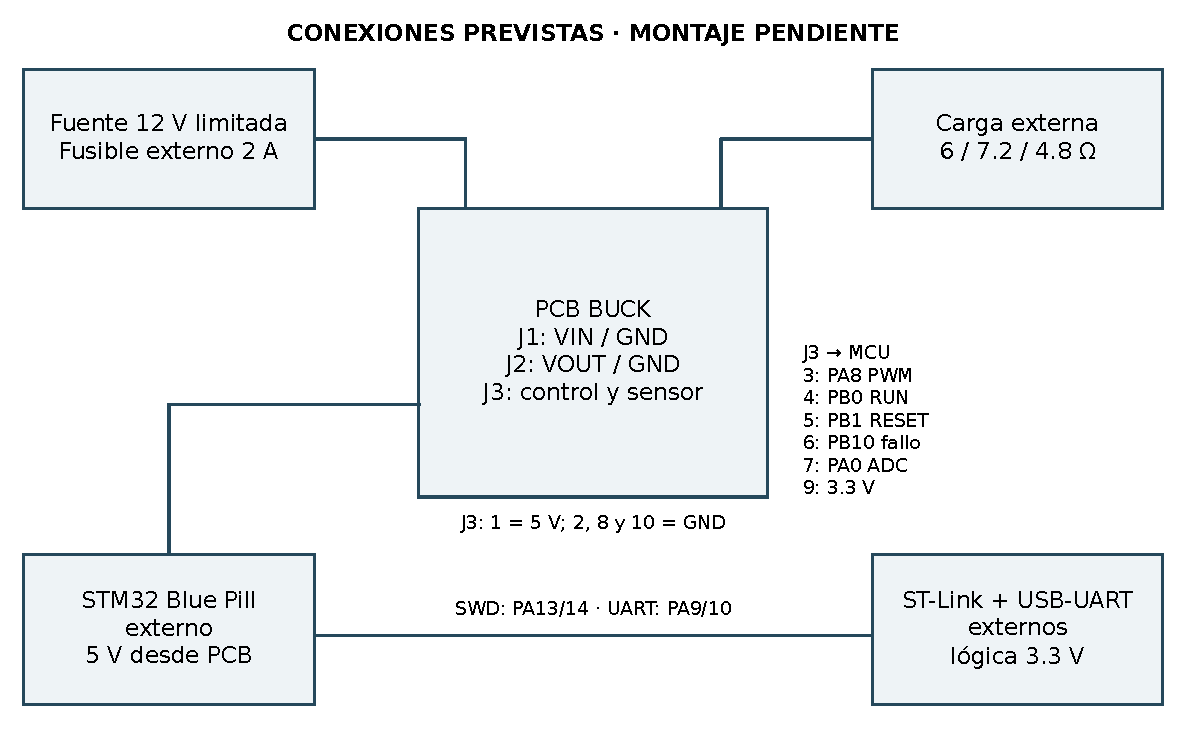
\includegraphics[width=\columnwidth]{assets/wiring.pdf}\caption{Interconexión prevista. MCU, programador, enlace serie y carga son externos a la PCB.}\label{fig:wiring}\end{figure}
TIM1 genera PWM por PA8 y sincroniza TIM3; este dispara ADC1/PA0 cada $5\,\mu\mathrm{s}$. DMA circular conserva dos bloques de 20 muestras. La interrupción TIM1 verifica bloque completo, promedia y precarga CCR para el siguiente periodo. La última conversión termina nominalmente a $97.667\,\mu\mathrm{s}$. DWT vigila ejecución y el watchdog exige adquisición fresca. Estos tiempos proceden de la configuración y deben medirse.

\begin{table}[H]\caption{Evidencia de implementación}\label{tab:implementation}\centering\footnotesize\setlength{\tabcolsep}{2pt}\renewcommand{\arraystretch}{1.18}\begin{tabularx}{\columnwidth}{LY}\toprule
Elemento & Estado\\\midrule
Compilación ARM & ELF, BIN y HEX generados\\
Núcleo y runtime C & Pruebas nativas y sanitizadores superadas\\
Captura serie & Cuatro pruebas automatizadas superadas\\
Programación / tiempo real & Pendiente en MCU\\
ADC / protección / térmica & Pendiente en laboratorio\\\bottomrule\end{tabularx}\end{table}
INA180A1 amplifica el shunt; LM393 activa un enclavamiento HCT00 por sobrecorriente o sobretensión. RUN bajo fuerza SD alto y deshabilita IR2110. El disparo tiene prioridad sobre RESET. Los umbrales nominales son 2 A y 8.2 V; la evaluación estática de tolerancias da 1.825--2.184 A y 7.561--8.868 V. Deben comprobarse retardo y disparo real. Se requiere fusible externo de 2 A y fuente limitada.

El enlace UART de 115200 baudios exporta las capturas después de detener RUN. Las 512 medias se guardan con duty aplicado y referencia; no equivalen al rizado instantáneo, que exige osciloscopio. Los escalones de carga manuales requieren captura con pretrigger. Conservar CSV crudos, calibración y versión de firmware junto a cada ensayo.

\section{Ensayos de aceptación}
Ejecutar por separado $r:6\to7\,\mathrm{V}$, $r:6\to5\,\mathrm{V}$, $R:6\to7.2\,\Omega$ y $R:6\to4.8\,\Omega$, estos últimos con $r=6\,\mathrm{V}$. Regresar al nominal y realizar tres repeticiones por caso. Capturar referencia, tensión, orden y carga desde $5\,\mathrm{ms}$ antes hasta al menos $20\,\mathrm{ms}$ después.

Usar $e_\infty=r_f-\operatorname{media}(\bar v_o)$ en una ventana final declarada. Medir $t_s$ con banda $\pm20\,\mathrm{mV}$ en referencia y $\pm0.12\,\mathrm{V}$ en carga. Medir sobreimpulso porcentual en referencia, pico $\max|\bar v_o-6|$ en carga y rizado instantáneo.

\begin{table}[H]\caption{Resultados físicos; P = pendiente}\label{tab:physical}\centering\footnotesize\setlength{\tabcolsep}{2pt}\renewcommand{\arraystretch}{1.18}\begin{tabularx}{\columnwidth}{LYYYY}\toprule
Caso & $t_s$ (ms) & $|e_\infty|$ (mV) & $M_p$/pico & Rizado (V)\\\midrule
$6\to7\,\mathrm{V}$ & P & P & P & P\\
$6\to5\,\mathrm{V}$ & P & P & P & P\\
$R:+20\%$ & P & P & P & P\\
$R:-20\%$ & P & P & P & P\\\bottomrule\end{tabularx}\end{table}
Agregar duty mínimo y máximo, corriente máxima, incertidumbre y dispersión. Comparar con la entrega 3 y explicar cuantización, latencia, pérdidas y saturación. Todo reajuste exige repetir los cuatro casos conservando el antes y después.

\section{Estado y conclusión experimental}
Faltan montaje identificado, firmware cargado en MCU, calibración, medición de temporización y apagado, y doce capturas mínimas. La simulación sustenta el ajuste inicial, pero no demuestra desempeño físico.

\appendices\section{Evidencia reproducible}\begingroup\raggedright
Conservar firmware, \texttt{buck\_control.c}, configuración de temporizador, calibración y CSV originales. El protocolo está en \texttt{project/hardware/implementacion.md}. El analizador compara el modelo promediado con duty y carga registrados; la evaluación del controlador debe añadir las métricas de aceptación y su incertidumbre.

\par\endgroup
\begin{thebibliography}{9}
\bibitem{guide}J. D. Bastidas Rodríguez, ``Proyecto de Curso: Convertidor Buck con control de tensión de salida, Universidad Nacional de Colombia, mayo 2025, pp. 1--3.
\end{thebibliography}\end{document}
